\chapter{Il livello di rete e i router}

\begin{center}
\begin{tikzpicture}[node distance=0pt]
  \node[lay app, minimum width=3.4cm] (a) {Applicazione};
  \node[lay tra, minimum width=3.4cm, below=of a] (t) {Trasporto};
  \node[lay net, minimum width=3.4cm, below=of t, line width=1.5pt, draw=netred] (n) {\bfseries Rete};
  \node[lay link, minimum width=3.4cm, below=of n] (l) {Collegamento};
  \node[lay phy, minimum width=3.4cm, below=of l] (p) {Fisico};
  \draw[-{Stealth}, thick, netred] ([xshift=0.3cm]n.east) -- ++(1,0) node[right, lbl, text=netred] {siamo qui};
\end{tikzpicture}
\end{center}

% ══════════════════════════════════════════════════════════════
\section{Dal trasporto alla rete}
% ══════════════════════════════════════════════════════════════

Per tre capitoli i mittenti hanno reagito a qualcosa che non potevano vedere: un timeout, tre conferme duplicate, una
finestra che si chiude, tutto in risposta a una perdita. E la perdita stessa era una curva, il ritardo di accodamento che
sale quando l'intensità di traffico si avvicina a uno, e poi pacchetti scartati. Nessuno ha mai aperto il nodo dove questo
succede: ora lo apriamo. Sotto il trasporto non ci sono più processi; questo livello sposta datagrammi da host a host, e
un suo pezzo gira in ogni router del percorso. Le domande sono due: come fa un datagramma che arriva da un collegamento a
uscire da quello giusto, e chi decide quale pacchetto parte per primo.

Il compito del livello di rete è permettere a host remoti di comunicare:

\begin{itemize}
    \item \textbf{sull'host mittente}: prendere i segmenti dal livello di trasporto, incapsulare ciascuno in un
          \textbf{datagramma} e inviare i datagrammi nella rete;
    \item \textbf{sull'host ricevente}: ricevere i datagrammi dalla rete, estrarne i segmenti di trasporto e
          consegnarli al livello di trasporto.
\end{itemize}

Fra i due non vale niente di ciò che abbiamo studiato finora: nessuna connessione, nessuna conferma, nessuna finestra.
A questo livello lavorano alcuni dei protocolli più importanti delle reti (IP, DHCP, NAT, ICMP, i protocolli di
routing) e i dispositivi che fanno di una rete una rete: i \textbf{router}. Il trasporto gira solo ai bordi; questo
livello gira \textbf{ovunque}, nei due host e in ogni router in mezzo, ed è per questo l'unico punto in cui tutta Internet
deve essere d'accordo.

\begin{figure}[H]
\centering
\begin{minipage}{0.45\linewidth}\centering
  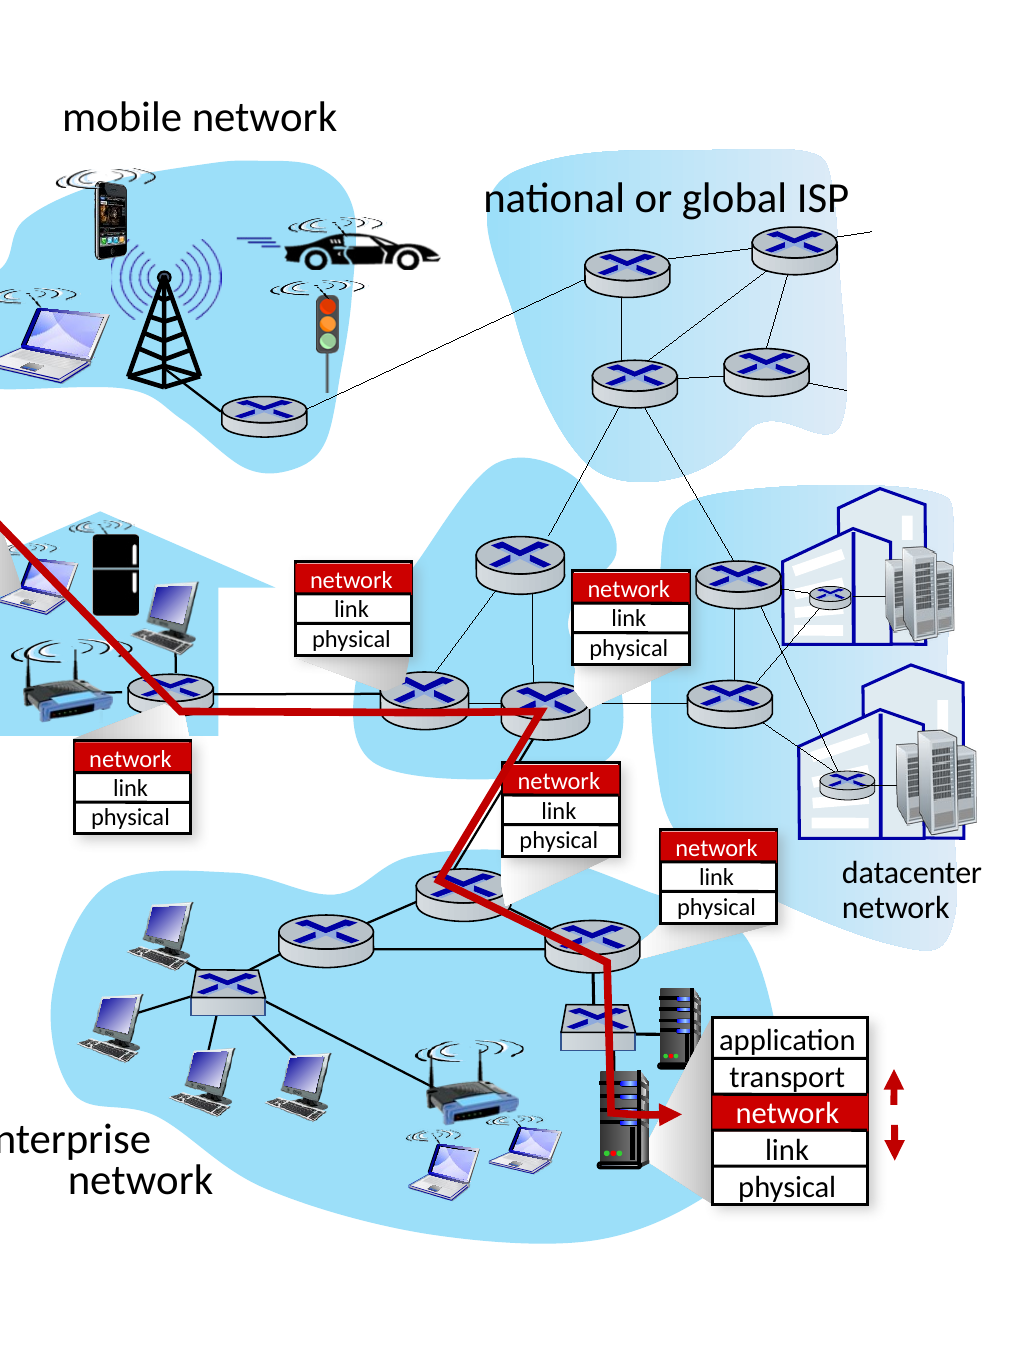
\includegraphics[width=0.9\linewidth]{cap13/stack_troncato.png}
\end{minipage}\hfill
\begin{minipage}{0.51\linewidth}
All'interno della rete ci sono nodi, i \textbf{router}, che inoltrano i datagrammi ai nodi adiacenti fino all'host
di destinazione.
\begin{itemize}
  \item Nelle figure i router hanno una \textbf{pila troncata} (rete, collegamento, fisico): non eseguono applicazioni
        né protocolli di trasporto.
  \item L'atto di un datagramma che viene reindirizzato da un router si chiama \textbf{hop} (salto).
\end{itemize}
\end{minipage}
\caption{Solo gli host hanno la pila completa; i router si fermano al livello di rete.}
\end{figure}

\begin{figure}[H]
\centering
\begin{tikzpicture}[every node/.style={font=\scriptsize\sffamily}]
  \begin{scope}
    \node[lay app, minimum width=1.8cm] at (0,2.4) {applicazione};
    \node[lay tra, minimum width=1.8cm] at (0,1.8) {trasporto};
    \node[lay net, minimum width=1.8cm] at (0,1.2) {rete};
    \node[lay link, minimum width=1.8cm] at (0,0.6) {collegamento};
    \node[lay phy, minimum width=1.8cm] at (0,0) {fisico};
    \node at (0,-0.6) {\icon[0.7cm]{pc}};
  \end{scope}
  \foreach \x/\n in {3.6/1, 7.2/2} {
    \begin{scope}[xshift=\x cm]
      \node[lay net, minimum width=1.8cm] at (0,1.2) {rete};
      \node[lay link, minimum width=1.8cm] at (0,0.6) {collegamento};
      \node[lay phy, minimum width=1.8cm] at (0,0) {fisico};
      \node at (0,-0.6) {\icon[0.9cm]{router}};
    \end{scope}
  }
  \begin{scope}[xshift=10.8cm]
    \node[lay app, minimum width=1.8cm] at (0,2.4) {applicazione};
    \node[lay tra, minimum width=1.8cm] at (0,1.8) {trasporto};
    \node[lay net, minimum width=1.8cm] at (0,1.2) {rete};
    \node[lay link, minimum width=1.8cm] at (0,0.6) {collegamento};
    \node[lay phy, minimum width=1.8cm] at (0,0) {fisico};
    \node at (0,-0.6) {\icon[0.4cm]{server}};
  \end{scope}
  \draw[-{Stealth}, very thick, netred] (0,2.1) -- (0,-0.25) -- (2.6,-0.25) -- (2.6,1.2) -- (4.6,1.2) -- (4.6,-0.25) -- (6.2,-0.25) -- (6.2,1.2) -- (8.2,1.2) -- (8.2,-0.25) -- (9.8,-0.25) -- (9.8,2.1);
  \node[text=netred] at (1.8,-1.1) {hop 1}; \node[text=netred] at (5.4,-1.1) {hop 2}; \node[text=netred] at (9,-1.1) {hop 3};
\end{tikzpicture}
\caption{Il datagramma sale fino al livello di rete in ogni router, che decide dove inoltrarlo, e riscende.}
\end{figure}

% ══════════════════════════════════════════════════════════════
\section{Che servizi offre il livello di rete}
% ══════════════════════════════════════════════════════════════

Il livello di rete è responsabile della \textbf{consegna host-a-host}. In teoria, insieme alla consegna potrebbe
offrire servizi come:

\begin{itemize}
    \item \textbf{consegna garantita}: un pacchetto inviato arriverà prima o poi a destinazione;
    \item \textbf{consegna garantita con ritardo limitato}: arriverà entro un certo tempo (per esempio 100 ms);
    \item \textbf{consegna in ordine}: i pacchetti arrivano nell'ordine di invio;
    \item \textbf{banda minima garantita}: se il mittente non supera una certa velocità (per esempio 1 Mb/s), tutti i
          pacchetti arrivano;
    \item \textbf{sicurezza}: cifratura e decifratura di tutti i datagrammi.
\end{itemize}

In realtà, \textbf{nessuno} di questi servizi è offerto in generale dalle reti.

\dfn{Servizio best effort}{
    Il livello di rete di Internet offre un solo servizio, detto \textbf{best effort} (``del proprio meglio''): la
    rete \textbf{fa del suo meglio} per consegnare un pacchetto dalla sorgente alla destinazione, ma non garantisce
    né che arrivi, né che arrivi in ordine, né ritardi massimi, né banda minima.
}

Suona come un eufemismo per «nessun servizio»: una rete che non consegnasse niente soddisferebbe la definizione. Altre
architetture facevano di più: \textbf{ATM} garantiva consegna in ordine, ritardo limitato e banda minima, e Internet non
le ha seguite. Nonostante la sua semplicità, il modello best effort, insieme a una buona disponibilità di banda e ad
applicazioni che si adattano, si è dimostrato \textbf{adeguato}: Netflix, le videochiamate, le conferenze in tempo reale
funzionano tutte così. E tutto ciò che di affidabile abbiamo scritto finora è costruito sopra di esso, dai due estremi,
partendo da niente.

% ══════════════════════════════════════════════════════════════
\section{I router nella rete}
% ══════════════════════════════════════════════════════════════

I router sono nodi speciali con \textbf{più collegamenti in ingresso e in uscita}. Offrono due funzioni di rete
fondamentali.

\dfn{Forwarding e routing}{
    \begin{itemize}
      \item \textbf{Forwarding} (inoltro): quando un pacchetto arriva su un collegamento di ingresso, il router lo
            sposta sul \textbf{collegamento di uscita} appropriato. È un'azione \textbf{locale} al router.
      \item \textbf{Routing} (instradamento): decidere il \textbf{percorso} che i pacchetti devono seguire dalla
            sorgente alla destinazione. È un processo che riguarda \textbf{tutta la rete}; gli algoritmi che
            calcolano i percorsi sono gli \textbf{algoritmi di routing}.
    \end{itemize}
}

Durante il forwarding un router può anche:

\begin{enumerate}
    \item \textbf{bloccare} un pacchetto (se proviene da un host noto come malevolo o è diretto a un host vietato);
    \item \textbf{scartare} un pacchetto scaduto;
    \item \textbf{duplicare} un pacchetto e inviarlo su più collegamenti;
    \item \textbf{modificare} un pacchetto (per esempio per segnalare congestione).
\end{enumerate}

\info{L'analogia del viaggio in auto}{
    Il \textbf{routing} è pianificare il viaggio da Napoli a Milano, scegliendo le autostrade da percorrere. Il
    \textbf{forwarding} è quello che si fa a ogni svincolo: guardare il cartello e imboccare l'uscita giusta. Il primo
    richiede una visione d'insieme e si fa una volta; il secondo è rapido, locale e si ripete a ogni incrocio.
}

\begin{figure}[H]
\centering
\begin{tikzpicture}[every node/.style={font=\footnotesize\sffamily}]
  \begin{scope}
    \node[font=\small\bfseries\sffamily] at (1.5,1.6) {Forwarding};
    \node (r) at (1.5,0) {\icon[1.3cm]{router}};
    \draw[msg, very thick, netblue] (-0.8,0.5) -- node[above] {P} (0.8,0.1);
    \draw[msg, very thick, netgreen] (2.2,0.1) -- (3.8,0.9); \draw[thick, black!30] (2.2,-0.1) -- (3.8,-0.8); \draw[thick, black!30] (0.8,-0.2) -- (-0.8,-0.8);
    \node[below=4pt of r, text width=3cm, align=center] {sposta il pacchetto dall'ingresso all'uscita giusta};
  \end{scope}
  \begin{scope}[xshift=7cm]
    \node[font=\small\bfseries\sffamily] at (2.5,1.6) {Routing};
    \foreach \x/\y [count=\i] in {0/0, 1.5/0.9, 1.6/-0.9, 3.2/0.6, 3.3/-0.7, 4.8/0} \node (n\i) at (\x,\y) {\icon[0.7cm]{router}};
    \foreach \a/\b in {1/2, 1/3, 2/4, 3/5, 2/5, 4/6, 5/6, 3/4} \draw[thick, black!30] (n\a) -- (n\b);
    \draw[pathhl, -{Stealth}] (n1) -- (n2) -- (n4) -- (n6);
    \node[text width=4.6cm, align=center] at (2.4,-1.8) {calcola il percorso migliore attraverso tutta la rete};
  \end{scope}
\end{tikzpicture}
\caption{Forwarding (locale) e routing (globale).}
\end{figure}

% ══════════════════════════════════════════════════════════════
\section{Tipi di router}
% ══════════════════════════════════════════════════════════════

\begin{figure}[H]
\centering
\begin{minipage}{0.4\linewidth}\centering
  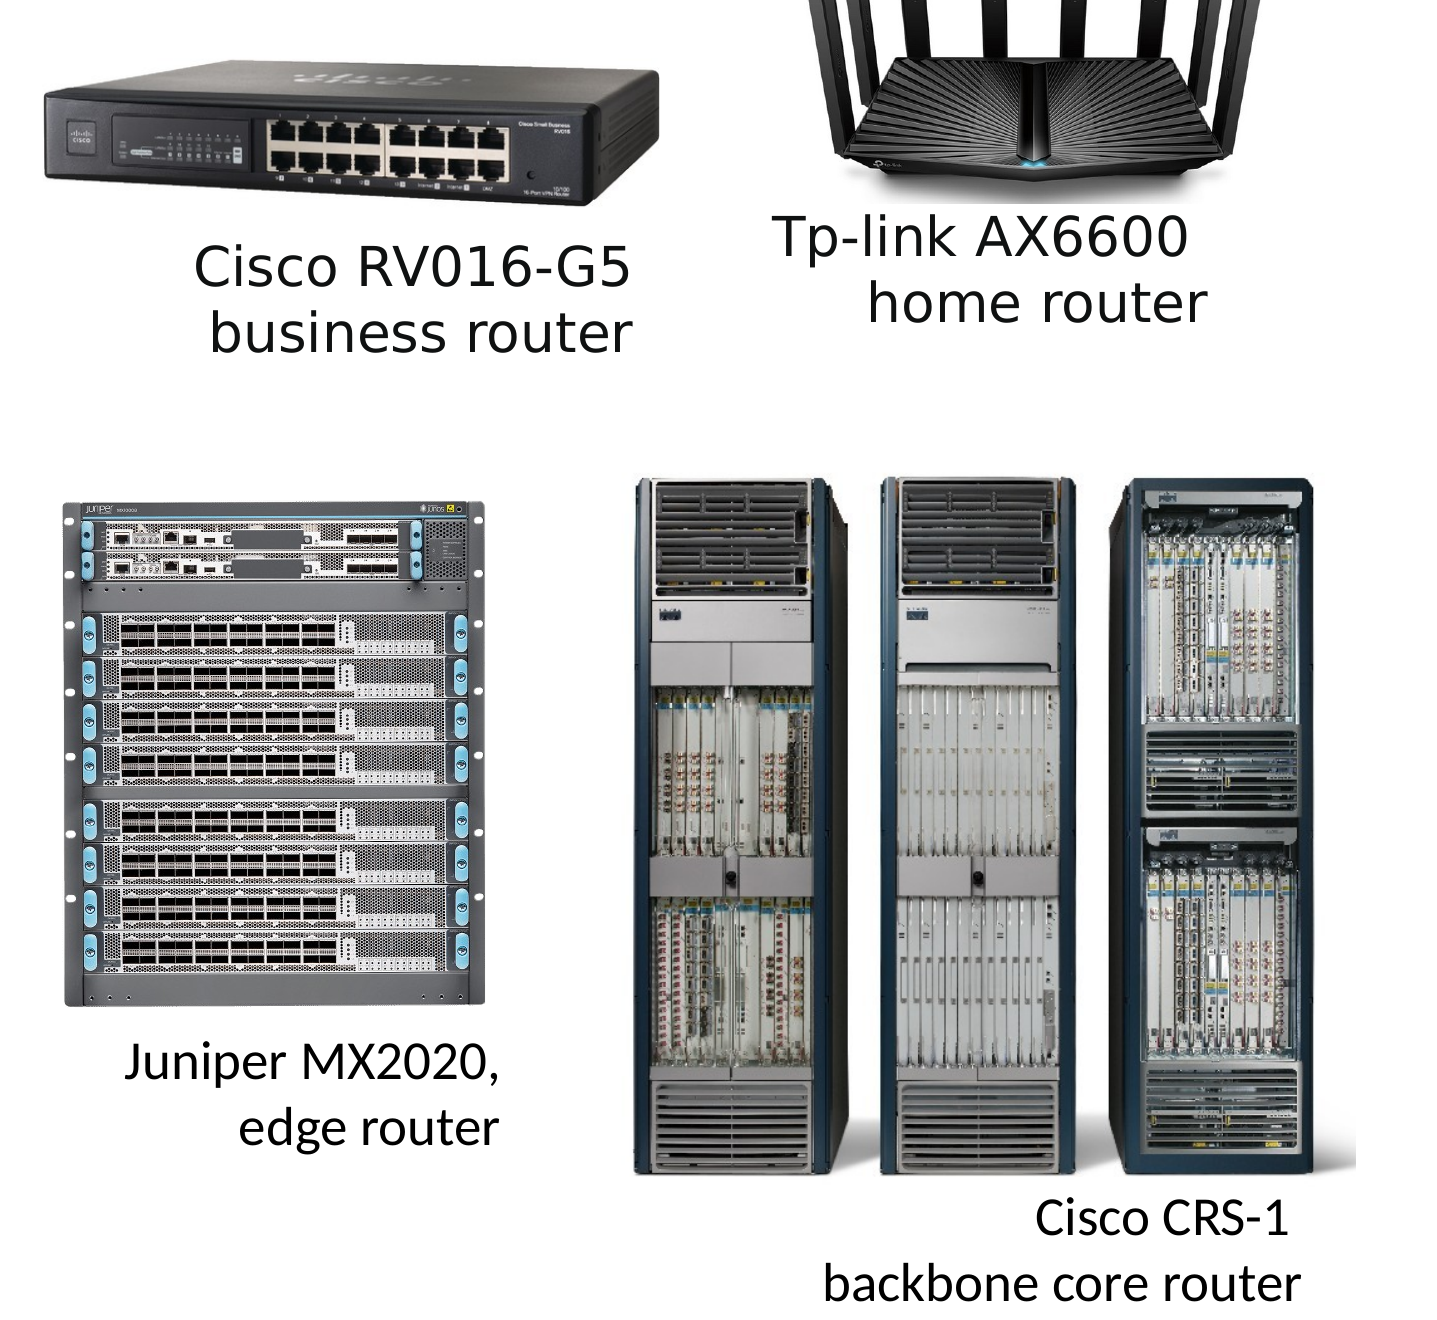
\includegraphics[width=0.95\linewidth]{cap13/router_foto.png}
\end{minipage}\hfill
\begin{minipage}{0.56\linewidth}
I router possono essere molto diversi a seconda di uso e tecnologia: per casa o per ufficio, con o senza fili.
Una distinzione importante è quella tra:
\begin{itemize}
  \item \textbf{edge router} (router di bordo): distribuiscono pacchetti \textbf{tra reti diverse}, per esempio
        collegando una rete con l'ISP. È il tipo più comune;
  \item \textbf{core router} (router di nucleo): distribuiscono pacchetti \textbf{all'interno di una stessa rete}.
        Sono usati anche sulla dorsale (\emph{backbone}) di Internet, dove devono smaltire trasferimenti di dati enormi.
\end{itemize}
\end{minipage}
\caption{Router per uso domestico e aziendale (in alto), un edge router e un core router da dorsale (in basso).}
\end{figure}

% ══════════════════════════════════════════════════════════════
\section{Data plane e control plane}
% ══════════════════════════════════════════════════════════════

\dfn{I due piani di un router}{
    \begin{itemize}
      \item Il \textbf{data plane} (piano dei dati, o di forwarding) comprende l'azione locale di trasferire un
            pacchetto da un'interfaccia di ingresso a quella di uscita appropriata. È un'operazione \textbf{veloce}
            (pochi nanosecondi), di solito realizzata in \textbf{hardware}.
      \item Il \textbf{control plane} (piano di controllo) comprende il processo, esteso a tutta la rete, che
            determina i percorsi da un estremo all'altro. È più \textbf{lento} (secondi), e spesso realizzato in
            \textbf{software}.
    \end{itemize}
}

Due funzioni su scale di tempo distanti un miliardo di volte: è per questo che hanno nomi separati. Fra le due sta una
sola struttura dati, la \textbf{forwarding table} (tabella di inoltro): il control plane la scrive, il data plane la legge
una volta per pacchetto. Associa gli indirizzi di destinazione ai collegamenti di uscita: il router inoltra un pacchetto
esaminando uno o più campi del suo header, e il valore trovato nella tabella indica l'interfaccia su cui inoltrarlo.
Conseguenza: un router inoltra \textbf{senza conoscere il percorso}; sa solo quale dei suoi collegamenti viene dopo.

\warning{La tabella non contiene i singoli indirizzi}{
    Una forwarding table \textbf{non} elenca gli indirizzi dei singoli host (sarebbero miliardi): associa alle porte
    di uscita \textbf{gruppi di indirizzi}, cioè intervalli individuati da un prefisso (le \emph{subnet}).
}

\subsection{Centralizzato o decentralizzato}

Poiché prima di arrivare a destinazione si attraversano molti router, il contenuto di una forwarding table va
determinato raccogliendo informazioni da router diversi. Lo si fa con una o più \textbf{tabelle di routing}
(control plane), da cui si ricava la forwarding table (data plane). Ci sono due modi:

\begin{figure}[H]
\centering
\begin{tikzpicture}[every node/.style={font=\scriptsize\sffamily}]
  \begin{scope}
    \node[font=\footnotesize\bfseries\sffamily] at (2.3,2.7) {Decentralizzato};
    \foreach \x [count=\i] in {0,1.5,3,4.5} {
      \node[draw, fill=lnet!40, minimum width=1.1cm, minimum height=0.5cm] (cp\i) at (\x,1.7) {routing};
      \node[draw, fill=llink!60, minimum width=1.1cm, minimum height=0.5cm] (dp\i) at (\x,0.9) {tabella};
      \draw[-{Stealth}] (cp\i) -- (dp\i);
      \node at (\x,0.1) {\icon[0.6cm]{router}};
    }
    \foreach \i/\j in {1/2, 2/3, 3/4} \draw[{Stealth}-{Stealth}, netred, thick] (cp\i) -- (cp\j);
    \node[text width=4.8cm, align=center] at (2.25,-0.7) {ogni router ha un componente di routing che dialoga con quelli degli altri};
  \end{scope}
  \begin{scope}[xshift=8cm]
    \node[font=\footnotesize\bfseries\sffamily] at (2.3,2.7) {Centralizzato (SDN)};
    \node[draw, fill=lnet!60, rounded corners, minimum width=4.8cm, minimum height=0.6cm] (ctrl) at (2.25,1.9) {controller remoto (software)};
    \foreach \x [count=\i] in {0,1.5,3,4.5} {
      \node[draw, fill=llink!60, minimum width=1.1cm, minimum height=0.5cm] (dp\i) at (\x,0.9) {tabella};
      \draw[-{Stealth}, netred, thick] (ctrl.south -| dp\i) -- (dp\i);
      \node at (\x,0.1) {\icon[0.6cm]{router}};
    }
    \node[text width=4.8cm, align=center] at (2.25,-0.7) {un controller separato calcola e distribuisce le tabelle di inoltro};
  \end{scope}
\end{tikzpicture}
\caption{Control plane decentralizzato e centralizzato.}
\end{figure}

\begin{itemize}
    \item \textbf{Decentralizzato} (distribuito): ogni router ha un componente di routing che comunica con i componenti
          di routing degli altri router. È stato a lungo l'approccio dominante.
    \item \textbf{Centralizzato}: un \textbf{controller remoto}, fisicamente separato dai router, calcola le tabelle e
          le distribuisce. Può trovarsi in un data center remoto, affidabile e ridondato, gestito dall'ISP o da terzi.
\end{itemize}

\info{Software-Defined Networking}{
    L'approccio centralizzato è alla base del \textbf{Software-Defined Networking} (SDN): la rete è ``definita dal
    software'' perché il controller che calcola le tabelle e dialoga con i router è un software centralizzato,
    talvolta anche open source. Si noti che cosa non cambia: il data plane delle due figure è identico, cambia solo
    l'autore della tabella.
}

% ══════════════════════════════════════════════════════════════
\section{Le componenti di un router}
% ══════════════════════════════════════════════════════════════

\begin{figure}[H]
\centering
\begin{tikzpicture}[every node/.style={font=\footnotesize\sffamily}]
  \draw[thick, rounded corners, fill=black!3] (-0.6,-3.3) rectangle (9.6,1.5);
  \node[anchor=north west, font=\small\bfseries\sffamily] at (-0.5,1.45) {Router};
  \foreach \y/\i in {0/1, -1.2/2, -2.6/N} {
    \node[draw, fill=lnet!40, minimum width=2cm, minimum height=0.8cm, align=center] (in\i) at (1,\y) {porta di\\ingresso \i};
    \node[draw, fill=llink!60, minimum width=2cm, minimum height=0.8cm, align=center] (out\i) at (8,\y) {porta di\\uscita \i};
    \draw[-{Stealth}, very thick] (-1.6,\y) -- (in\i.west);
    \draw[-{Stealth}, very thick] (out\i.east) -- (10.6,\y);
  }
  \node at (1,-1.9) {$\vdots$}; \node at (8,-1.9) {$\vdots$};
  \node[draw, fill=ltra!50, minimum width=2.4cm, minimum height=3.4cm, align=center] (sf) at (4.5,-1.3) {switching\\fabric};
  \foreach \i in {1,2,N} { \draw[-{Stealth}, thick] (in\i.east) -- (in\i.east -| sf.west); \draw[-{Stealth}, thick] (out\i.west -| sf.east) -- (out\i.west); }
  \node[draw, fill=lapp!50, rounded corners, minimum width=3cm, align=center] (rp) at (4.5,2.4) {processore di routing\\(control plane)};
  \draw[{Stealth}-{Stealth}, dashed, thick, netred] (rp.south) -- node[right, text=netred] {tabelle} (sf.north);
  \draw[-{Stealth}, dashed, netred] (rp.west) -| (in1.north);
  \node[anchor=east] at (-1.7,-1.3) {collegamenti di ingresso};
  \node[anchor=west, text width=2cm] at (10.7,-1.3) {collegamenti di uscita};
  \node[text=black!60] at (4.5,-3.0) {data plane (hardware)};
\end{tikzpicture}
\caption{Architettura di un router.}
\end{figure}

\begin{itemize}
    \item \textbf{Porte di ingresso} (da non confondere con le porte del trasporto, i numeri a 16 bit: queste sono
          interfacce fisiche) collegate ai collegamenti in ingresso. Il loro compito è:
    \begin{itemize}
      \item terminare il collegamento fisico e fare il lavoro di livello di collegamento necessario a parlare con l'altro
            capo;
      \item consultare la forwarding table (\emph{lookup}) e preparare la switching fabric verso la porta di uscita scelta;
      \item inoltrare al processore di routing i pacchetti di controllo (per esempio quelli con le informazioni di routing);
      \item controllare versione, checksum e \emph{time-to-live} del datagramma, riscrivere gli ultimi due, e aggiornare i
            contatori di gestione.
    \end{itemize}
    Il numero di porte va da decine a centinaia: il Juniper MX2020 arriva a 800 porte da 100 Gb/s in un solo chassis.
    È la scala a distinguere un router di casa da uno di dorsale, non la funzione.
    \item \textbf{Switching fabric} (matrice di commutazione): collega le porte di ingresso a quelle di uscita.
    \item \textbf{Porte di uscita}: conservano i pacchetti ricevuti dalla switching fabric e li trasmettono sul
          collegamento in uscita. Le porte possono essere bidirezionali (ingresso e uscita accoppiati).
    \item \textbf{Processore di routing}: esegue i protocolli di routing, mantiene informazioni sullo stato dei
          collegamenti e calcola e aggiorna la forwarding table.
\end{itemize}

\info{Perché il lookup non può essere software}{
    Un collegamento in ingresso da 100 Gb/s e un datagramma da 64 byte: la porta ha \textbf{5,12 ns} prima che possa
    arrivare il successivo. Le schede di linea portano più porte insieme, e allora tutta la catena deve girare $N$ volte
    più in fretta. Nessun software ci si avvicina: porte di ingresso, porte di uscita e fabric sono hardware, progettato dal
    costruttore o comprato come silicio. Il processore di routing sta all'altro capo della scala, su millisecondi e secondi,
    e può essere una normale CPU con normale codice. È la forma di tutto il livello: la parte veloce è stupida e ripetitiva,
    quella intelligente è lenta e rara.
}

% ══════════════════════════════════════════════════════════════
\section{Il forwarding e la longest prefix matching}
% ══════════════════════════════════════════════════════════════

La forwarding table associa \textbf{indirizzi IP} a \textbf{porte di uscita}, così che i pacchetti possano essere
inoltrati sul collegamento giusto verso il nodo successivo (dove, eventualmente, verranno inoltrati di nuovo).

Un indirizzo IP è un numero di \textbf{4 byte} (32 bit), che di solito si scrive in notazione decimale ma che si può
vedere in binario:

\begin{center}
\begin{tabular}{ll}
decimale puntata & \texttt{192.168.1.1} \\
binario & \texttt{11000000 10101000 00000001 00000001} \\
\end{tabular}
\end{center}

Quando un pacchetto arriva su una porta di ingresso si esegue un \textbf{lookup}. Ogni porta ha una
\textbf{copia} della forwarding table, ricevuta dal processore di routing su un bus dedicato (per esempio PCI), per
evitare il collo di bottiglia di interrogare il processore per ogni pacchetto. Più indirizzi possono essere
associati alla stessa porta.

\warning{Una riga per indirizzo è fuori discussione}{
    Che cosa c'è di sbagliato nell'elencare semplicemente gli indirizzi? Una riga per ogni destinazione possibile sono
    $2^{32}$ righe, più di quattro miliardi, in ogni router, da cercare in nanosecondi; e andrebbero riscritte ogni volta
    che un host compare o sparisce da qualche parte. Quindi una riga non nomina un indirizzo: nomina un \textbf{gruppo di
    indirizzi che condividono i primi bit}, una subnet.
}

Ogni riga fissa i primi bit e lascia liberi gli altri: la parte fissa nomina il gruppo, quella libera un host al suo
interno. La prima riga della tabella seguente fissa 21 bit; gli 11 liberi danno $2^{11} = 2048$ indirizzi, da tutti zeri
a tutti uni. Una riga è quindi un \textbf{intervallo}, e quattro righe sostituiscono quattro miliardi. L'ultima,
\emph{altrimenti}, è il \textbf{default}: ciò che non corrisponde a niente deve comunque uscire da qualche parte.

\begin{table}[H]
\centering
\begin{tabular}{llc}
\toprule
\textbf{Prefisso degli indirizzi} & \textbf{Intervallo di indirizzi corrispondente} & \textbf{Interfaccia} \\
\midrule
\texttt{11001000 00010111 00010*** ********} & da \texttt{...00010000 00000000} a \texttt{...00010111 11111111} & 0 \\
\texttt{11001000 00010111 00011000 ********} & da \texttt{...00011000 00000000} a \texttt{...00011000 11111111} & 1 \\
\texttt{11001000 00010111 00011*** ********} & da \texttt{...00011000 00000000} a \texttt{...00011111 11111111} & 2 \\
altrimenti & & 3 \\
\bottomrule
\end{tabular}
\caption{Una forwarding table a 4 porte: ogni riga è un prefisso, cioè un intervallo di indirizzi (i primi 16 bit sono sempre \texttt{11001000 00010111}).}
\end{table}

\warning{Righe che si sovrappongono}{
    Le righe non sono necessariamente mutuamente esclusive. Per esempio l'indirizzo
    \texttt{11001000 00010111 00011000 10101010} corrisponde sia alla riga dell'interfaccia 1 sia a quella
    dell'interfaccia 2. A quale porta va?
}

\dfn{Longest prefix matching}{
    Se un indirizzo corrisponde a più righe della forwarding table, il router lo inoltra verso la porta associata alla
    riga con il \textbf{prefisso più lungo} (\emph{longest prefix matching rule}).
}

\begin{figure}[H]
\centering
\begin{tikzpicture}[every node/.style={font=\small\ttfamily}]
  \node[anchor=west] (addr) at (0,0) {\textcolor{netred}{11001000 00010111 00011000} 10101010};
  \node[anchor=west, font=\small\sffamily] at (8,0) {indirizzo di destinazione};
  \draw[decorate, decoration={brace, amplitude=5pt}, netgreen!60!black, thick] (0.1,0.35) -- (6.05,0.35) node[midway, above=6pt, font=\footnotesize\sffamily, text=netgreen!50!black] {match con la riga dell'interfaccia 1: 24 bit};
  \draw[decorate, decoration={brace, amplitude=5pt, mirror}, netblue, thick] (0.1,-0.35) -- (5.35,-0.35) node[midway, below=6pt, font=\footnotesize\sffamily, text=netblue] {match con la riga dell'interfaccia 2: 21 bit};
  \node[font=\small\bfseries\sffamily, text=netgreen!50!black] at (10,-1.1) {vince l'interfaccia 1!};
\end{tikzpicture}
\caption{Longest prefix matching: tra le righe che corrispondono si sceglie quella con il prefisso più lungo.}
\end{figure}

\begin{esempio}{Dove va il pacchetto?}
Con la tabella precedente:
\begin{itemize}
    \item \texttt{11001000 00010111 00010110 10100001}: corrisponde solo al prefisso \texttt{...00010} $\Rightarrow$ interfaccia \textbf{0};
    \item \texttt{11001000 00010111 00011000 10101010}: corrisponde a \texttt{...00011000} (24 bit) e a \texttt{...00011} (21 bit)
          $\Rightarrow$ interfaccia \textbf{1};
    \item \texttt{11001000 00010111 00011001 00000001}: corrisponde solo a \texttt{...00011} $\Rightarrow$ interfaccia \textbf{2};
    \item \texttt{11001000 00010111 00100000 00000001}: nessun prefisso $\Rightarrow$ interfaccia \textbf{3}.
\end{itemize}
\end{esempio}

Il confronto avviene solo sui bit del prefisso e si ferma dove il prefisso finisce; i bit che avanzano dicono quale host
dentro il gruppo, e al router non servono. È il senso di tutta l'organizzazione: un router in un altro continente ha bisogno
di conoscere il gruppo, mai la macchina.

\begin{esempio}{Ritagliare un blocco da un blocco}
Due righe di una forwarding table:
\begin{center}
\begin{tabular}{l l c}
\toprule
\textbf{Prefisso} & \textbf{Lunghezza} & \textbf{Porta} \\
\midrule
\texttt{11001000 00010111 00011000} \texttt{********} & 24 bit & 1 (verso l'Europa) \\
\texttt{11001000 00010111 00011000 01}\texttt{******} & 26 bit & 2 (verso le Americhe) \\
\bottomrule
\end{tabular}
\end{center}
Arriva un pacchetto per \texttt{11001000 00010111 00011000 01001101}: corrisponde a entrambe, e la corrispondenza a 26 bit
è la più lunga, quindi vince la porta 2. Le due righe descrivono lo stesso blocco da 24 bit; la seconda ne prende un
quarto (due bit in più) e lo manda altrove. Senza la regola le due righe si contraddirebbero; con la regola dicono
«tutto questo blocco di là, \textbf{tranne} questo pezzo». È così che si sposta un cliente senza rinumerare nessuno.
\end{esempio}

\info{Il lookup in nanosecondi}{
    Come problema è semplice: trovare la riga corrispondente più lunga. A velocità di gigabit va risolto in nanosecondi,
    quindi non solo in hardware, ma con qualcosa di meglio di una scansione lineare. Il vincolo che plasma il progetto è il
    tempo di accesso alla memoria: DRAM integrata nel chip, SRAM più veloce come cache davanti. Oppure la \textbf{TCAM}
    (\emph{ternary content-addressable memory}): si presentano i 32 bit alla memoria e restituisce la riga in tempo
    praticamente costante; i dispositivi grandi ne contengono dell'ordine di un milione.
}

Determinata la porta di uscita, il pacchetto entra nella switching fabric; se altre porte stanno usando la fabric, può
dover attendere in coda.

\subsection{Match-plus-action}

L'operazione in due passi ``cerca l'indirizzo di destinazione'' (\emph{match}) e ``inoltra'' (\emph{action}) si
chiama \textbf{match-plus-action} ed è eseguita in molti dispositivi di rete:

\begin{itemize}
    \item \textbf{switch}: azione simile a quella dei router (ma su indirizzi di livello 2);
    \item \textbf{firewall}: l'azione è filtrare, cioè bloccare, certi pacchetti in arrivo;
    \item \textbf{NAT} (\emph{Network Address Translator}): l'azione è riscrivere indirizzo e porta di certi pacchetti prima di inoltrarli.
\end{itemize}
Tre dispositivi che il corso incontra separatamente, a fare una sola cosa in tre costumi: vale la pena riconoscerli quando
compaiono.

% ══════════════════════════════════════════════════════════════
\section{La switching fabric}
% ══════════════════════════════════════════════════════════════

\begin{figure}[H]
\centering
\begin{tikzpicture}[every node/.style={font=\scriptsize\sffamily}]
  \begin{scope}
    \node[font=\footnotesize\bfseries\sffamily] at (1.6,2.4) {1. Memoria};
    \foreach \y [count=\k] in {1.5,0.5,-0.5} { \node[draw, fill=lnet!40, minimum width=0.8cm] (i\k) at (0,\y) {in}; \node[draw, fill=llink!60, minimum width=0.8cm] (o\k) at (3.2,\y) {out}; }
    \node[draw, fill=ltra!50, minimum width=1.2cm, minimum height=2.6cm, align=center] (mem) at (1.6,0.5) {CPU\\+\\memoria};
    \draw[-{Stealth}, netred, thick] (i1) -- (mem); \draw[-{Stealth}, netred, thick] (mem) -- (o3);
    \node[text width=3.6cm, align=center] at (1.6,-1.5) {il processore copia il pacchetto: lento, tipico dei primi router};
  \end{scope}
  \begin{scope}[xshift=5.6cm]
    \node[font=\footnotesize\bfseries\sffamily] at (1.6,2.4) {2. Bus};
    \foreach \y in {1.5,0.5,-0.5} { \node[draw, fill=lnet!40, minimum width=0.8cm] at (0,\y) {in}; \node[draw, fill=llink!60, minimum width=0.8cm] at (3.2,\y) {out}; \draw (0.4,\y) -- (2.8,\y); }
    \draw[line width=4pt, netblue] (1.6,1.9) -- (1.6,-0.9);
    \draw[-{Stealth}, netred, very thick] (0.4,1.5) -- (1.6,1.5) -- (1.6,-0.5) -- (2.8,-0.5);
    \node[text width=3.6cm, align=center] at (1.6,-1.5) {bus condiviso: una porta alla volta, basta per reti piccole};
  \end{scope}
  \begin{scope}[xshift=11.2cm]
    \node[font=\footnotesize\bfseries\sffamily] at (1.6,2.4) {3. Rete di interconnessione};
    \foreach \y in {1.5,0.5,-0.5} { \node[draw, fill=lnet!40, minimum width=0.8cm] at (0,\y) {in}; \draw (0.4,\y) -- (2.6,\y); }
    \foreach \x in {1.0,1.6,2.2} { \draw (\x,1.9) -- (\x,-0.9); \node[draw, fill=llink!60, minimum width=0.5cm, rotate=90] at (\x,-1.1) {\tiny out}; }
    \foreach \x in {1.0,1.6,2.2} \foreach \y in {1.5,0.5,-0.5} \fill[black!40] (\x,\y) circle (1.5pt);
    \draw[netred, very thick, -{Stealth}] (0.4,1.5) -- (2.2,1.5) -- (2.2,-0.8);
    \draw[netgreen!60!black, very thick, -{Stealth}] (0.4,-0.5) -- (1.0,-0.5) -- (1.0,-0.8);
    \node[text width=3.6cm, align=center] at (1.6,-1.9) {punti di incrocio che si aprono e chiudono: più pacchetti in parallelo};
  \end{scope}
\end{tikzpicture}
\caption{I tre modi di realizzare la commutazione.}
\end{figure}

\begin{enumerate}
    \item \textbf{Commutazione tramite memoria}: le porte sono trattate come dispositivi di I/O; un pacchetto in arrivo
          interrompe il processore, viene copiato in memoria, cercato nella tabella e copiato nel buffer della porta di
          uscita. Il pacchetto attraversa la memoria \textbf{due volte}: se la memoria regge $B$ pacchetti al secondo, il
          router ne inoltra meno di $B/2$. E due pacchetti non possono essere inoltrati insieme nemmeno verso porte diverse,
          perché sul bus condiviso passa una lettura o una scrittura alla volta. Era il modo dei primi router, che erano
          normali computer; i router moderni a memoria condivisa fanno lookup e scrittura sulla scheda di linea, non in una
          CPU centrale.
    \item \textbf{Commutazione tramite bus}: la porta di ingresso trasferisce il pacchetto direttamente alla porta di uscita
          su un bus condiviso, senza intervento del processore. Gli antepone un'etichetta interna che nomina la porta di
          uscita: tutte le porte vedono il pacchetto, solo quella nominata lo tiene, e toglie l'etichetta. Un pacchetto alla
          volta sul bus: la velocità di commutazione del router è quella del bus. Spesso basta (un noto router aziendale di
          questo tipo commuta su un bus da 32 Gb/s): semplice, economico, e con un tetto rigido.
    \item \textbf{Commutazione tramite rete di interconnessione} (\emph{crossbar}): $2N$ bus collegano $N$ ingressi a $N$
          uscite, con un punto di incrocio a ogni intersezione che si apre e si chiude. Per portare un pacchetto da A a Y il
          controllore chiude l'incrocio AY, e solo il bus Y lo raccoglie; così A$\to$Y e B$\to$X avvengono
          \textbf{insieme}, cosa che le altre due non possono fare. È \textbf{non bloccante}: un pacchetto non viene mai
          fermato sulla strada verso una porta di uscita che nessun altro sta usando. Ma due pacchetti per la stessa porta
          si contendono ancora, e uno aspetta in ingresso.
\end{enumerate}

% ══════════════════════════════════════════════════════════════
\section{Le code sulle porte}
% ══════════════════════════════════════════════════════════════

Poiché la commutazione richiede tempo, porte di ingresso e di uscita hanno \textbf{code} (buffer) in cui i pacchetti
aspettano, come le auto a un semaforo. L'entità delle code non è fissa: dipende dal carico di traffico, dalla velocità
della switching fabric e da quella delle linee. In generale i pacchetti possono arrivare o partire più velocemente o
più lentamente di quanto avvenga la commutazione, e accumularsi in un buffer di ingresso o di uscita, che può
\textbf{traboccare}.

\begin{esempio}{Dove si formano le code}
Un router ha $N$ porte di ingresso e $N$ di uscita; tutte le linee hanno velocità $R_{line}$ pacchetti al secondo e tutte
le porte ricevono pacchetti contemporaneamente. Nel caso peggiore \textbf{tutti} i pacchetti vanno alla \textbf{stessa}
porta di uscita. Detta $R_{switch}$ la velocità della switching fabric:
\begin{itemize}
    \item se $R_{switch} \approx N \cdot R_{line}$: la fabric smaltisce tutto in tempo, le code in \textbf{ingresso} sono
          trascurabili, ma quella in \textbf{uscita} cresce, perché arrivano $N$ volte più pacchetti di quanti il collegamento ne trasmetta;
    \item se $R_{line} < R_{switch} < N \cdot R_{line}$: si formano code \textbf{su entrambe} le porte (l'ingresso aspetta la
          fabric, l'uscita aspetta il collegamento);
    \item se $R_{switch} \approx R_{line}$: la coda in uscita è trascurabile, ma quelle in \textbf{ingresso} sono consistenti.
\end{itemize}
\end{esempio}

Letti insieme, i tre casi dicono che nessuna scelta di fabric elimina l'accodamento: decide solo \textbf{dove} avviene.

\warning{Head-of-the-line blocking}{
    La fabric è non bloccante. Perché allora un pacchetto si ferma? Perché una coda di ingresso è servita \textbf{in
    ordine}: il pacchetto in testa aspetta una porta di uscita occupata, e tutto ciò che sta dietro aspetta con lui,
    compreso un pacchetto la cui porta sarebbe libera. È il \emph{blocco in testa alla coda} (HOL blocking): da solo fa
    crescere la coda di ingresso senza limite già quando il ritmo di arrivo raggiunge circa il \textbf{58\%} della capacità
    della linea. È uno dei motivi per cui le code in ingresso vanno evitate.
}

\subsection{Quando non c'è più posto}

\begin{itemize}
    \item Anche con una fabric $N$ volte più veloce delle linee, $N$ pacchetti possono raggiungere una porta di uscita nel
          tempo che serve a inviarne uno: le code in uscita si formano comunque.
    \item Quando la memoria è finita le scelte sono due: scartare il pacchetto che arriva (\textbf{drop-tail}), o fare
          posto togliendo pacchetti già in coda. Un pacchetto lascia la coda solo quando è stato trasmesso per intero: fino ad
          allora occupa il suo buffer.
    \item Può anche convenire scartare, o \textbf{marcare}, prima che il buffer sia pieno, come avvertimento al mittente: sono
          le politiche di \key{gestione attiva della coda} (AQM), di cui la più nota è \textbf{RED}. E marcare invece di
          scartare è proprio ciò a cui servivano i due bit ECN nell'header: è questa la macchina che li accende.
\end{itemize}

\subsection{Quanto buffer basta}

\begin{itemize}
    \item La regola pratica per anni: buffer $=$ RTT medio $\times$ capacità del collegamento. Un collegamento da 10 Gb/s con
          250 ms vuole 2,5 Gbit di buffer.
    \item Quella cifra viene dall'analisi di pochi flussi TCP. Con $N$ flussi numerosi e indipendenti il requisito scende a
          $\text{RTT} \cdot C / \sqrt{N}$: nel nucleo, dove migliaia di flussi condividono un collegamento, è una riduzione
          enorme.
    \item E di più non è meglio: un buffer più grande assorbe raffiche più grandi e allunga il ritardo di accodamento di tutto
          ciò che contiene. Dieci volte il buffer per evitare perdite può significare dieci volte il ritardo da un capo
          all'altro, e un'andata e ritorno più lunga rende ogni mittente su quel percorso più lento a reagire.
\end{itemize}

\begin{esempio}{La coda che non si svuota mai}
Un router di casa impiega 20 ms a inviare un pacchetto, l'andata e ritorno è di 200 ms, e a $t = 0$ una raffica di 25
pacchetti arriva in coda; c'è un solo flusso, nessun altro traffico.
\begin{itemize}
    \item A $t = 200$ ms arriva la prima conferma, proprio mentre parte il ventunesimo pacchetto, e libera un nuovo pacchetto
          nella coda.
    \item A $t = 220$ ms arriva la successiva, e un altro pacchetto entra in coda: uno dentro per ognuno fuori, finché dura il
          trasferimento.
    \item La coda si assesta a cinque pacchetti e ci resta. Il tubo è pieno, il throughput è esattamente giusto, e il ritardo è
          costante, grande, e causato soltanto dal buffer: $5 \times 20 = 100$ ms in più a ogni andata e ritorno.
\end{itemize}
\end{esempio}

\dfn{Bufferbloat}{
    Il \textbf{bufferbloat} è il ritardo permanente causato da buffer troppo grandi che restano pieni. Nessuno si comporta
    male: il mittente fa ciò per cui è stato progettato, e a essere sbagliato è il buffer.
}

% ══════════════════════════════════════════════════════════════
\section{La schedulazione dei pacchetti}
% ══════════════════════════════════════════════════════════════

È normale che più pacchetti, anche da porte di ingresso diverse, debbano uscire dalla stessa porta. L'accesso dei
pacchetti in coda al collegamento di uscita va quindi \textbf{schedulato}. I tre approcci più noti sono:

\begin{itemize}
    \item \textbf{FIFO} (\emph{First-In-First-Out}, o FCFS, \emph{First-Come-First-Served}): basato sull'ordine di arrivo;
    \item \textbf{a priorità} (\emph{priority queuing}): basato sull'importanza dei pacchetti;
    \item \textbf{round-robin}: i pacchetti sono divisi in classi, servite a turno.
\end{itemize}

\begin{figure}[H]
\centering
\begin{tikzpicture}[every node/.style={font=\scriptsize\sffamily}]
  \begin{scope}
    \node[font=\footnotesize\bfseries\sffamily] at (1.3,2.2) {FIFO};
    \draw[thick] (0,0) -- (0,1.5) -- (2.6,1.5); \draw[thick] (0,0) -- (2.6,0); \draw[thick] (2.6,0) -- (2.6,1.5);
    \foreach \x/\n in {0.3/3, 1.1/2, 1.9/1} { \fill[netblue!50] (\x,0.4) rectangle ++(0.5,0.7); \node at (\x+0.25,0.75) {\n}; }
    \draw[-{Stealth}, very thick] (-1,0.75) -- (0,0.75); \draw[-{Stealth}, very thick] (2.6,0.75) -- (3.6,0.75) node[right] {collegamento};
    \node[text width=3.4cm, align=center] at (1.3,-0.7) {esce per primo chi è arrivato per primo; a coda piena si scarta l'ultimo arrivato (\emph{drop-tail})};
  \end{scope}
  \begin{scope}[xshift=5.8cm]
    \node[font=\footnotesize\bfseries\sffamily] at (1.3,2.2) {Priorità};
    \foreach \y/\c/\t in {1.0/netred/alta, 0/netblue/bassa} {
      \draw[thick] (0,\y) rectangle (2.2,\y+0.7);
      \foreach \x in {1.0,1.6} \fill[\c!50] (\x,\y+0.1) rectangle ++(0.45,0.5);
      \node[anchor=east] at (-0.1,\y+0.35) {\t};
      \draw[-{Stealth}, thick] (2.2,\y+0.35) -- (2.9,0.85);
    }
    \node[circle, draw, fill=white] (sw) at (3.1,0.85) {};
    \draw[-{Stealth}, very thick] (sw) -- (4,0.85);
    \node[text width=3.6cm, align=center] at (1.6,-0.7) {si serve sempre la classe più importante non vuota; dentro la classe si va in FIFO};
  \end{scope}
  \begin{scope}[xshift=11.4cm]
    \node[font=\footnotesize\bfseries\sffamily] at (1.3,2.2) {Round-robin / WFQ};
    \foreach \y/\c/\t in {1.0/netgreen/{classe 1 (peso 2)}, 0/netorange/{classe 2 (peso 1)}} {
      \draw[thick] (0,\y) rectangle (2.2,\y+0.7);
      \foreach \x in {1.0,1.6} \fill[\c!50] (\x,\y+0.1) rectangle ++(0.45,0.5);
      \node[anchor=south] at (1.1,\y+0.7) {\t};
      \draw[-{Stealth}, thick] (2.2,\y+0.35) -- (2.9,0.85);
    }
    \node[circle, draw, fill=white] (sw) at (3.1,0.85) {};
    \draw[-{Stealth}, very thick] (sw) -- (4,0.85);
    \draw[-{Stealth}, netred] (3.1,1.35) arc (90:-200:0.5);
    \node[text width=3.6cm, align=center] at (1.6,-0.7) {le classi si alternano; con WFQ ogni classe ha un peso che ne fissa la quota};
  \end{scope}
\end{tikzpicture}
\caption{Tre politiche di schedulazione della coda di uscita.}
\end{figure}

In ogni caso un pacchetto viene tolto solo quando è stato trasmesso per intero: la scelta si fa alla fine di ogni
trasmissione, non di continuo.

\subsection{FIFO (First-Come-First-Served)}

\begin{itemize}
    \item Se il collegamento di uscita è occupato, i pacchetti in arrivo alla porta di uscita vengono \textbf{bufferizzati}.
    \item Se non c'è spazio sufficiente, serve una politica di scarto: la più comune è scartare il pacchetto appena arrivato
          (\textbf{drop-tail}); in approcci più sofisticati si possono rimuovere anche pacchetti già in coda per fare posto ai nuovi.
    \item Un pacchetto viene tolto dalla coda solo quando è stato \textbf{completamente trasmesso}.
    \item I pacchetti vengono trasmessi nello stesso ordine in cui sono arrivati: nessun pacchetto può essere favorito, e
          nessuno ritardato a vantaggio di un altro. È il default proprio per questo: non c'è niente da configurare e niente
          da sbagliare.
\end{itemize}

\subsection{Priority queuing}

\begin{itemize}
    \item All'arrivo in coda i pacchetti vengono \textbf{classificati} in classi di priorità (per esempio in base alle porte TCP/UDP).
    \item Un operatore può configurare la coda perché alcuni pacchetti (informazioni di gestione della rete, voce su IP in
          tempo reale, \dots) abbiano priorità sul traffico degli utenti o non in tempo reale.
    \item Ogni classe ha la propria coda: si trasmettono per primi i pacchetti della classe \textbf{più prioritaria non vuota};
          dentro una stessa classe si procede in FIFO.
    \item È \textbf{non preemptive}: una trasmissione già cominciata non viene mai interrotta, e un pacchetto ad alta
          priorità che arriva a metà aspetta comunque che finisca.
\end{itemize}

\subsection{Round-robin queuing}

\begin{itemize}
    \item I pacchetti sono ancora divisi in classi, ma le classi vengono \textbf{alternate} invece che scelte per priorità.
    \item È \textbf{work-conserving}: non lascia mai il collegamento inattivo, e una classe con la coda vuota viene saltata
          subito.
    \item Un'implementazione comune è il \textbf{Weighted Fair Queuing} (WFQ): i pacchetti vengono classificati e accodati
          nella propria area di attesa, e a ogni classe $i$ è associato un \textbf{peso} $w_i$. Una classe con pacchetti da
          inviare riceve una quota $w_i / \sum_j w_j$ del servizio, quindi su un collegamento di rate $R$ ha garantito almeno
          \[ R \cdot \frac{w_i}{\sum_j w_j} \]
          qualunque cosa facciano le altre; la priorità stretta, invece, alla classe bassa non garantisce niente.
\end{itemize}

\begin{figure}[H]
\centering
\begin{tikzpicture}[x=0.62cm, every node/.style={font=\scriptsize\sffamily},
    pk/.style={draw=black!60, minimum height=0.45cm, minimum width=1.24cm, anchor=west, font=\scriptsize\bfseries\sffamily},
    hi/.style={pk, fill=netblue!25}, lo/.style={pk, fill=netorange!30}]
  \node[anchor=east] at (-0.4,0) {arrivi};
  \foreach \t/\n in {0/1, 0.5/2, 1/3, 1.5/4, 10/5} {
    \draw[-{Stealth[length=1.5mm]}, thick] (\t,0.45) -- (\t,0.05);
    \node[above] at (\t,0.45) {\n};
  }
  \node[anchor=east, align=right] at (-0.4,-0.9) {FIFO};
  \foreach \t/\n in {0/1, 2/2, 4/3, 6/4, 10/5} \node[pk, fill=black!8] at (\t,-0.9) {\n};
  \node[anchor=east, align=right] at (-0.4,-1.8) {priorità\\\tiny alta 1 3 4, bassa 2 5};
  \node[hi] at (0,-1.8) {1}; \node[hi] at (2,-1.8) {3}; \node[hi] at (4,-1.8) {4}; \node[lo] at (6,-1.8) {2}; \node[lo] at (10,-1.8) {5};
  \node[anchor=east, align=right] at (-0.4,-2.7) {round robin\\\tiny classe 1: 1 2 4, classe 2: 3 5};
  \node[hi] at (0,-2.7) {1}; \node[lo] at (2,-2.7) {3}; \node[hi] at (4,-2.7) {2}; \node[hi] at (6,-2.7) {4}; \node[lo] at (10,-2.7) {5};
  \foreach \r in {-0.9,-1.8,-2.7} \node[text=black!50] at (9,\r) {inattivo};
  \draw[-{Stealth[length=2mm]}] (0,-3.3) -- (13,-3.3) node[right]{tempo};
  \foreach \t in {0,2,...,12} { \draw (\t,-3.25) -- (\t,-3.35); \node[below] at (\t,-3.35) {\t}; }
\end{tikzpicture}
\caption{Stessi arrivi, tre ordini di partenza (ogni trasmissione dura 2 unità). Con la priorità 3 e 4 superano 2, che era
         arrivato prima di entrambi e parte ultimo dei quattro. Con il round robin 3 parte presto perché alla sua classe
         spettava un turno, mentre 4 non supera 2, che è della stessa classe. Il collegamento resta inattivo prima del 5 in
         tutti e tre: uno scheduler decide un ordine, non crea mai capacità.}
\end{figure}

\info{Chi decide che cos'è una classe}{
    Il meccanismo è neutro. Che cosa conta come classe lo decide chi gestisce la rete, su qualsiasi campo dell'header: una
    porta ben nota (la gestione prima della posta), o un indirizzo sorgente (il traffico di un'azienda che ha pagato prima
    di quello di una che non l'ha fatto). Lo stesso match-plus-action può anche bloccare il traffico di una certa azienda,
    o di un certo paese. I limiti qui sono quindi \textbf{legali} più che tecnici, e cambiano da paese a paese: è il tema
    della \key{neutralità della rete}. Le regole statunitensi del 2015 vietavano blocco, rallentamento e priorità a
    pagamento, e nel 2017 sono state sostituite da obblighi di trasparenza; nell'Unione Europea il regolamento 2015/2120
    vieta blocchi e rallentamenti discriminatori. La questione torna, dal lato del denaro, quando ci si chiede perché due
    reti accettino di trasportare l'una il traffico dell'altra.
}

\Needspace{20\baselineskip}
% ══════════════════════════════════════════════════════════════
\section{Riepilogo}
% ══════════════════════════════════════════════════════════════

\riepilogo{
\begin{itemize}
    \item Il livello di rete consegna datagrammi \textbf{da host a host}, con servizio \textbf{best effort}.
    \item I router fanno \textbf{forwarding} (locale, data plane, hardware, nanosecondi) e \textbf{routing} (globale, control
          plane, software, secondi); il control plane può essere distribuito o centralizzato (SDN).
    \item Un router ha porte di ingresso, switching fabric (memoria, bus, crossbar), porte di uscita e processore di routing.
    \item La forwarding table associa \textbf{prefissi} a interfacce; vince il \textbf{prefisso più lungo}.
    \item Le code si formano dovunque un rate incontra un rate più lento, in ingresso, in uscita o in entrambi: è lì che
          nasce la perdita che i mittenti deducono. Buffer troppo grandi non la eliminano, la trasformano in ritardo
          (bufferbloat).
    \item La schedulazione può essere FIFO, a priorità (non preemptive) o round-robin (WFQ, con una quota garantita per
          classe). Resta da vedere da dove vengono gli indirizzi dentro quei prefissi.
\end{itemize}
}
